% ============================================================
% Section « Modélisation et expérimentation » (version avec formules)
% Packages nécessaires dans le préambule :
%   \usepackage{amsmath, amssymb}
%   \usepackage{tabularx, setspace, float}
% ============================================================

\section{Modélisation et expérimentation}

\subsection{Architecture du système}

\begin{figure}[H]
\centering
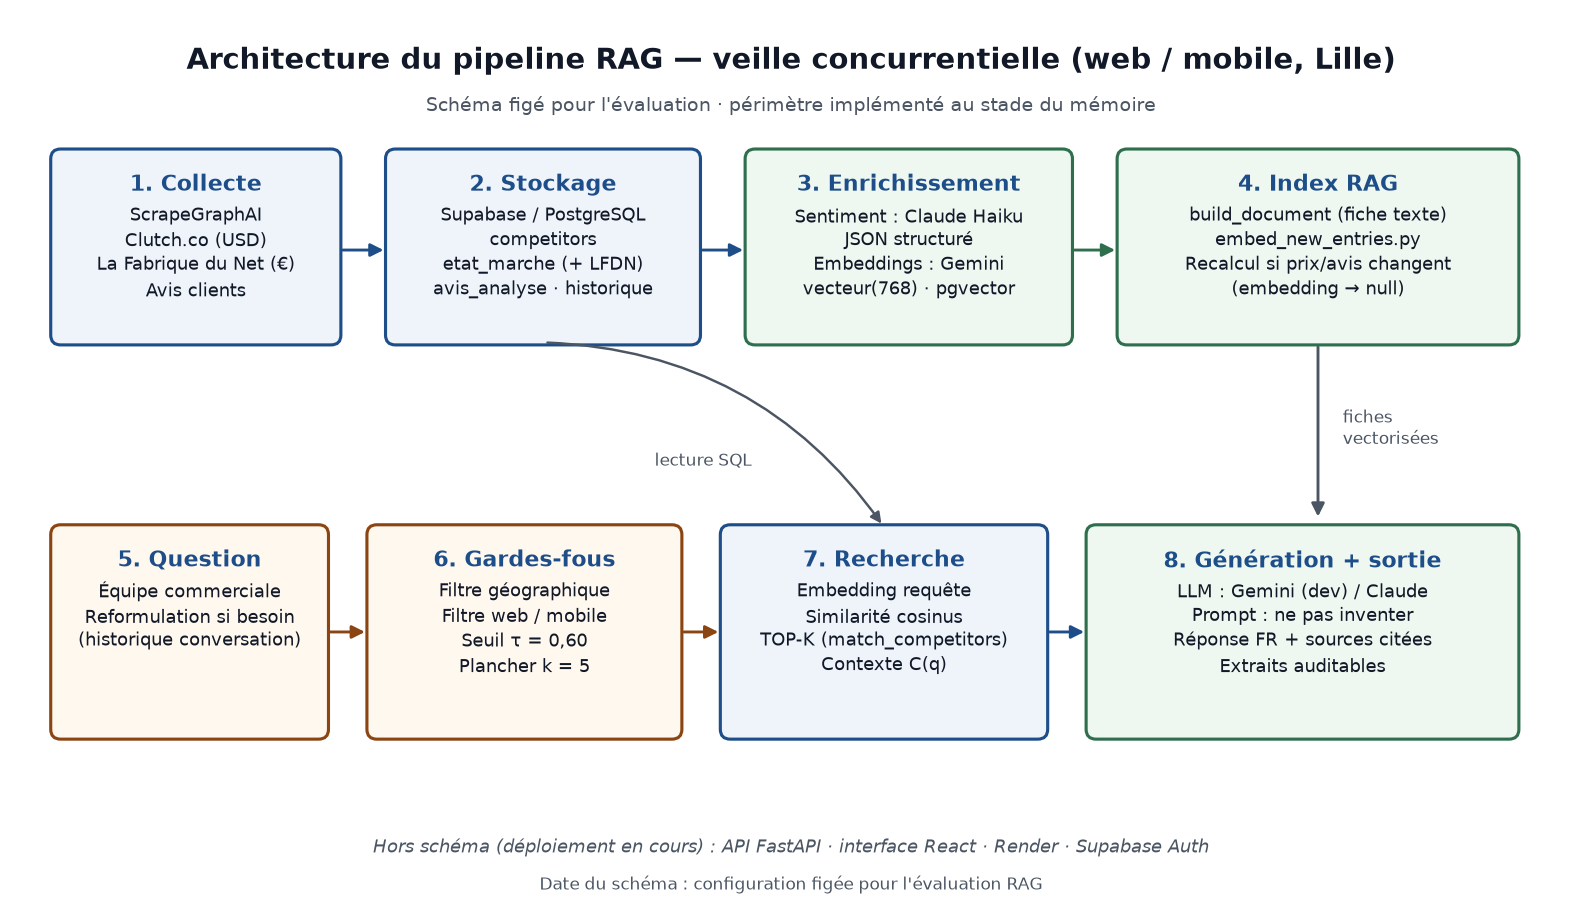
\includegraphics[width=0.95\textwidth]{img/architecture_rag.png}
\caption{Schéma d'architecture du pipeline RAG.
Flux~: collecte (ScrapeGraphAI) $\rightarrow$ stockage Supabase $\rightarrow$ analyse de sentiment (Claude) $\rightarrow$ embeddings (Gemini) $\rightarrow$ recherche vectorielle (\texttt{pgvector}) $\rightarrow$ génération de réponse (Gemini/Claude) $\rightarrow$ restitution sources.
Date du schéma~: configuration figée pour l'évaluation.
Périmètre~: composants effectivement implémentés au stade du mémoire (hors interface React/API FastAPI si non finalisées).
Exclusion~: services tiers non critiques (quota API, détails d'hébergement Render) omis pour la lisibilité.}
\label{fig:architecture_rag}
\end{figure}

\subsection{Pourquoi ce projet ne relève pas de l'apprentissage supervisé}

Le besoin exprimé par l'entreprise n'est pas de prédire une classe ou une valeur numérique. L'équipe
commerciale pose des questions en français sur ses concurrents : fourchettes de prix, avis clients,
comparaison entre offres web et mobile, informations sur une agence nommée. La réponse doit s'appuyer sur des
fiches déjà collectées et signaler explicitement les cas où ces fiches ne suffisent pas.

Un modèle de régression, de classification ou de clustering ajusterait ses paramètres $\theta$ en minimisant
une fonction de perte sur un jeu de données annoté $\{(x_i, y_i)\}_{i=1}^{n}$ :
\begin{equation}
    \hat{\theta} = \operatorname*{arg\,min}_{\theta} \; \frac{1}{n} \sum_{i=1}^{n} \mathcal{L}\big(f_{\theta}(x_i),\, y_i\big)
    \label{eq:supervise}
\end{equation}
Or un tel jeu n'existe pas : il n'y a ni centaines de questions étiquetées « bonne » ou « mauvaise »
réponse, ni avis annotés manuellement. Entraîner un modèle de langue, voire affiner un modèle comme
CamemBERT, aurait exigé des données et un temps de calcul que la durée du stage ne permettait pas. L'approche
retenue relève donc du \textit{transfert} : des modèles préentraînés, dont les paramètres $\theta$ restent
figés, sont appelés par API, et le travail de modélisation porte sur la manière de les articuler.

Le système construit est une architecture RAG (\textit{Retrieval-Augmented Generation}). Une question est
convertie en vecteur, comparée aux fiches des concurrents, puis un modèle de langue rédige la réponse à partir
des seules fiches retrouvées. Il n'y a donc aucune phase d'apprentissage des poids : le travail se décompose
en une phase de construction du pipeline, suivie d'une phase d'évaluation sur un jeu de questions fixé à
l'avance.

\subsection{Sélection des modèles}

Trois tâches ont été distinguées, car elles n'impliquent ni le même coût ni le même besoin de nuance.

\textbf{Recherche.} Chaque fiche concurrent est convertie en vecteur par le modèle
\texttt{gemini-embedding-2}, dont la dimension est fixée à 768 afin de rester alignée sur la colonne
\texttt{vector(768)} de Supabase. Deux modes d'utilisation du même modèle sont distingués :
\texttt{retrieval\_document} lors de l'indexation d'une fiche et \texttt{retrieval\_query} lors de
l'encodage d'une question. La comparaison repose sur la similarité cosinus, calculée par \texttt{pgvector} via
la fonction SQL \texttt{match\_competitors}.

Formellement, chaque texte $x$ (fiche ou question) est transformé par le modèle d'embedding en un vecteur
$\mathbf{e}(x) \in \mathbb{R}^{768}$. Lorsque la dimension est réduite de 3\,072 à 768 composantes, le vecteur
tronqué n'est plus de norme unitaire ; il est donc normalisé :
\begin{equation}
    \hat{\mathbf{e}}(x) = \frac{\mathbf{e}(x)}{\lVert \mathbf{e}(x) \rVert_2}
    \label{eq:norme}
\end{equation}
La proximité entre une question $q$ et une fiche $d$ est ensuite mesurée par la similarité cosinus :
\begin{equation}
    s(q, d) = \cos\big(\mathbf{e}(q), \mathbf{e}(d)\big)
    = \frac{\mathbf{e}(q) \cdot \mathbf{e}(d)}{\lVert \mathbf{e}(q) \rVert \, \lVert \mathbf{e}(d) \rVert}
    = \frac{\sum_{i=1}^{768} q_i \, d_i}
           {\sqrt{\sum_{i=1}^{768} q_i^{2}} \; \sqrt{\sum_{i=1}^{768} d_i^{2}}}
    \label{eq:cosine}
\end{equation}
avec $s(q,d) \in [-1, 1]$ ; plus la valeur est proche de 1, plus les deux textes sont sémantiquement proches.
L'avantage de cette mesure est qu'elle ne dépend que de l'angle entre les vecteurs, et non de leur norme. Pour
des vecteurs normalisés, elle se réduit au simple produit scalaire $s(q,d) = \hat{\mathbf{e}}(q) \cdot \hat{\mathbf{e}}(d)$.

Dans \texttt{pgvector}, l'opérateur \texttt{<=>} renvoie la distance cosinus
\begin{equation}
    d_{\cos}(q,d) = 1 - s(q,d)
    \label{eq:distance}
\end{equation}
et la fonction \texttt{match\_competitors} reconvertit ce résultat en similarité par $s = 1 - d_{\cos}$.

\textbf{Rédaction de la réponse.} Le modèle de chat est interchangeable. En développement,
\texttt{gemini-3.1-flash-lite} permet de limiter le coût et la consommation de quota. Pour la soutenance, le
même appel peut basculer vers Claude Sonnet (\texttt{claude-sonnet-4-5b}, 1\,000 jetons maximum) en
modifiant la variable \texttt{LLM\_PROVIDER}, sans changement dans le reste du pipeline.

\textbf{Analyse des avis, en amont du RAG.} Les avis ne sont pas traités par un classifieur entraîné. Claude
Haiku (\texttt{claude-haiku-4-5}) produit, en une seule passe et sans exemple annoté, un JSON au format imposé
comprenant le sentiment global, un score et des thèmes :
\begin{equation}
    \text{sentiment} \in \{\text{positif},\ \text{neutre},\ \text{négatif}\}, \qquad
    \sigma \in [0, 1], \qquad
    T \subseteq \mathcal{T}
    \label{eq:avis}
\end{equation}
où $\sigma$ est le score de sentiment et $\mathcal{T}$ la liste fermée des thèmes (délais, communication,
qualité, prix, réactivité, expertise technique). Un classifieur classique n'aurait fourni qu'une étiquette,
alors que l'objectif était de produire également des points forts et des points faibles directement
réutilisables dans la fiche.

Les tâches légères, comme la reformulation d'une question de suivi (« et pour le mobile ? ») ou le résumé de
l'historique de conversation, restent confiées au modèle Gemini le plus léger, même lorsque la réponse
finale est générée par Claude.

\subsection{Construction du système}

Le pipeline n'apprend pas : il prépare des documents, les indexe une fois pour toutes, puis les retrouve à
chaque question.

\subsubsection{Préparation et indexation des fiches}

Une fiche est un texte court construit par la fonction \texttt{build\_document}. Elle réunit le nom de
l'entreprise, le type de prestation (web ou mobile), la source (Clutch ou La Fabrique du Net), les tarifs
disponibles (budget minimum, taux horaire, coût moyen ou fourchette), puis au plus quatre points forts et
quatre points faibles issus de l'analyse des avis. Lorsque cette analyse n'existe pas, la fiche l'indique
explicitement. Le champ « thèmes », plus verbeux, n'est pas recopié : il répétait les informations déjà
présentes et alourdissait inutilement le contexte transmis au modèle.

Ces textes sont vectorisés une seule fois par le script \texttt{embed\_new\_entries.py}, et uniquement pour
les lignes dont l'embedding est vide. Tout changement de prix ou toute nouvelle analyse d'avis remet
l'embedding à \texttt{null}, ce qui déclenche un recalcul ciblé. Au moment de la question, le système ne
ré-encode donc jamais la base.

\subsubsection{Formalisation du traitement d'une question}

Soit $\mathcal{D}$ l'ensemble des fiches indexées. Pour une question $q$, le système construit un ensemble de
contexte $\mathcal{C}(q)$, puis le modèle de langue génère la réponse $r$ à partir de cet unique contexte :
\begin{equation}
    r \sim p_{\text{LLM}}\big(\,\cdot \mid q,\ \mathcal{C}(q)\big)
    \label{eq:rag}
\end{equation}
L'ensemble $\mathcal{C}(q)$ est obtenu en quatre temps.

\textbf{(i) Voisins les plus proches.} On classe les fiches par similarité décroissante,
$s(q, d_{(1)}) \ge s(q, d_{(2)}) \ge \dots \ge s(q, d_{(|\mathcal{D}|)})$, puis on retient les $K = 12$
premières :
\begin{equation}
    \mathcal{N}_{K}(q) = \big\{\, d_{(1)},\, d_{(2)},\, \dots,\, d_{(K)} \,\big\}
    \label{eq:topk}
\end{equation}

\textbf{(ii) Filtre web/mobile.} Soit $t(q) \in \{\text{web}, \text{mobile}\}$ le type de prestation détecté
dans la question, lorsqu'il est univoque, et $\operatorname{type}(d)$ celui de la fiche $d$ :
\begin{equation}
    \mathcal{N}'_{K}(q) =
    \begin{cases}
        \{\, d \in \mathcal{N}_{K}(q) : \operatorname{type}(d) = t(q) \,\} & \text{si ce sous-ensemble est non vide,} \\[4pt]
        \mathcal{N}_{K}(q) & \text{sinon.}
    \end{cases}
    \label{eq:filtre}
\end{equation}

\textbf{(iii) Seuil de similarité.} Avec le seuil $\tau = 0{,}60$ :
\begin{equation}
    \mathcal{S}(q) = \big\{\, d \in \mathcal{N}'_{K}(q) \;:\; s(q,d) \ge \tau \,\big\}
    \label{eq:seuil}
\end{equation}

\textbf{(iv) Plancher.} Avec $k = 5$ le nombre de fiches fournies au modèle :
\begin{equation}
    \mathcal{C}(q) =
    \begin{cases}
        \varnothing
        & \text{si } |\mathcal{S}(q)| = 0, \\[4pt]
        \text{les } k \text{ premières fiches de } \mathcal{N}'_{K}(q)
        & \text{si } 0 < |\mathcal{S}(q)| < k, \\[4pt]
        \text{les } k \text{ meilleures fiches de } \mathcal{S}(q)
        & \text{si } |\mathcal{S}(q)| \ge k.
    \end{cases}
    \label{eq:plancher}
\end{equation}
Dans le deuxième cas, les fiches ajoutées dont la similarité est inférieure à $\tau$ sont marquées
« confiance faible ». On note $\mathcal{F}(q) = \{\, d \in \mathcal{C}(q) : s(q,d) < \tau \,\}$ l'ensemble de
ces fiches ; le prompt précise que l'échantillon ne représente pas l'ensemble du marché dès que
\begin{equation}
    |\mathcal{F}(q)| > \frac{|\mathcal{C}(q)|}{2}
    \label{eq:faible}
\end{equation}

\subsubsection{Traitement d'une question à l'exécution}

À l'exécution, la fonction \texttt{ask} enchaîne cinq étapes.

\begin{enumerate}
    \item \textbf{Filtre géographique.} Si la question cite une ville connue hors de la zone couverte (Paris,
    Lyon, Tokyo, etc.) sans mentionner Lille ni les Hauts-de-France, la recherche s'arrête et un message
    indique que la base ne couvre pas cette zone. Ce filtre est volontairement incomplet : il complète la
    consigne du prompt sans la remplacer.
    \item \textbf{Recherche vectorielle.} La question est encodée, puis les 12 voisins les plus proches sont
    demandés à la base (équation~\ref{eq:topk}).
    \item \textbf{Filtre web/mobile.} Si la question porte clairement sur le web ou sur le mobile, et non sur
    les deux, les fiches de l'autre type sont écartées. Si ce filtre vide la liste, il est annulé
    (équation~\ref{eq:filtre}).
    \item \textbf{Seuil de similarité et plancher.} Les voisins dont la similarité cosinus est inférieure à
    0,60 sont écartés. S'il en reste au moins un mais moins de cinq, la liste est complétée jusqu'à cinq
    fiches, et ces compléments sont marqués « confiance faible ». S'il n'en reste aucun, la liste demeure
    vide : c'est le cas d'une question hors sujet, pour laquelle forcer des fiches produirait une réponse
    inventée (équations~\ref{eq:seuil} et~\ref{eq:plancher}).
    \item \textbf{Génération.} Les fiches retenues sont injectées dans un prompt qui interdit d'inventer,
    impose de signaler les informations manquantes et rappelle que la base porte sur le développement web et
    mobile à Lille. Si plus de la moitié des fiches sont en confiance faible (équation~\ref{eq:faible}), le
    prompt précise que l'échantillon ne représente pas l'ensemble du marché (69 fiches dans le texte du
    prompt).
\end{enumerate}

En conversation, une question de type « et lui ? » est d'abord reformulée à partir de l'historique, afin que
la recherche reçoive une phrase autonome. En l'absence de pronom ou de formulation en « et\ldots », la
question n'est pas réécrite.

\subsection{Paramètres retenus}

Il n'y a pas de validation croisée au sens statistique, puisqu'aucun poids n'est ajusté sur des plis. Les
réglages ont été fixés par essais successifs, en observant les questions pour lesquelles le système se
trompait.

\begin{table}[H]
\centering
\begingroup
\setstretch{1.1}
\small
\begin{tabularx}{\textwidth}{|p{4.2cm}|p{3.4cm}|X|}
\hline
\textbf{Paramètre} & \textbf{Valeur retenue} & \textbf{Rôle} \\
\hline
Dimension des vecteurs & $768$ & Aligne l'API et la colonne \texttt{pgvector}. Sans ce forçage, l'API renvoie
3\,072 dimensions. \\
\hline
Voisins demandés à la base ($K$) & $12$ & Laisse de la marge avant le filtre web/mobile et le seuil. \\
\hline
Nombre de fiches fournies au modèle ($k$) & $5$ & Assez pour comparer, sans noyer la réponse. \\
\hline
Seuil de similarité cosinus ($\tau$) & $0{,}60$ & En dessous, la fiche n'est pas considérée comme une vraie
correspondance. \\
\hline
Plancher & $k = 5$, seulement si $\lvert\mathcal{S}(q)\rvert \ge 1$ & Évite qu'une question large
(« la concurrence à Lille ») ne renvoie qu'un seul nom, sans rouvrir la porte aux questions hors sujet. \\
\hline
Jetons de la réponse Claude & $1\,000$ & Borne la longueur de la réponse commerciale. \\
\hline
\end{tabularx}
\endgroup
\caption{Paramètres retenus pour la configuration finale du pipeline RAG}
\label{tab:parametres}
\end{table}

Le seuil $\tau = 0{,}60$ est le réglage le plus sensible. Trop bas, une question sur la météo ou sur Tokyo
récupère malgré tout des agences, car les mots « prix » et « application » ressemblent à ceux des fiches.
Trop haut, une question générale ne ramène presque aucune fiche et donne l'impression que la base est vide.
Le plancher de cinq fiches ne s'applique que lorsqu'au moins une fiche dépasse le seuil, c'est-à-dire lorsque
$|\mathcal{S}(q)| \ge 1$ : c'est ce qui distingue une question vague mais pertinente d'une question hors sujet.

Le filtre géographique a été ajouté à la suite d'observations sur le jeu de
développement (19 questions). Sur une question du type « prix d'une application
mobile à Tokyo », la similarité restait élevée et le modèle respectait ou non
la consigne du prompt selon les exécutions. Le filtre par liste de villes rend
ce cas déterministe, sans appel au modèle. Ces ajustements (seuil, filtre)
ayant été réalisés après observation des échecs sur ce même ensemble de
questions, celui-ci est désormais traité comme un jeu de développement et non
comme un test final indépendant.

\subsection{Protocole d'évaluation}

\subsubsection{Séparation développement / test}

Deux jeux de questions sont distingués.

Le jeu de développement $Q_{\text{dev}}$ compte $|Q_{\text{dev}}| = 19$ questions.
Il a servi au réglage du seuil $\tau$, du filtre géographique et à l'analyse des
échecs. Il n'est plus utilisé pour rapporter les performances finales.

Le jeu de test indépendant $Q$ (cible $|Q| = 60$) est construit après figement
des modèles, prompts, filtres et paramètres. Les réponses et sources attendues
sont définies avant exécution. Il se répartit en familles :
\begin{itemize}
    \item $Q_{\text{pert}}$ : questions pertinentes (prix, sentiment, nominatives) ;
    \item $Q_{\text{hs}}$ : questions hors sujet, pour lesquelles aucune fiche
    ne doit être renvoyée ;
    \item questions hors zone géographique ;
    \item questions hors couverture métier (prestation ou information absente
    des fiches).
\end{itemize}

On note $Q_{\text{vt}} \subset Q_{\text{pert}}$ le sous-ensemble des questions
dont le concurrent attendu $d^{*}_q$ est connu à l'avance, et $\mathcal{C}(q)$
la liste des sources effectivement renvoyées pour la question $q$.

\subsubsection{Portée des métriques automatiques}

L'\textit{accuracy}, le score F1, l'AUC et la RMSE ne constituent pas les
métriques principales : il n'y a ni classe binaire apprise, ni erreur numérique
à minimiser. Les métriques calculées par \texttt{evaluate\_rag.py} diagnostiquent
le comportement de la recherche ; elles ne mesurent pas, à elles seules, la
véracité ni la complétude de la réponse générée.

\begin{itemize}
    \item \textbf{Comportement de retrieval attendu.} Pour une question
    pertinente, au moins une source est renvoyée. Pour une question hors sujet,
    aucune source. Pour une question hors zone, aucune source ou uniquement des
    sources sous le seuil. Pour une question hors couverture, aucune source ou
    une réponse indiquant explicitement que l'information n'est pas disponible.
    Si $b(q) \in \{0,1\}$ désigne cet indicateur :
    \begin{equation}
        \text{Comportement retrieval} =
        \frac{1}{|Q|} \sum_{q \in Q} b(q)
        \label{eq:comportement}
    \end{equation}
    Ce taux a une définition étroite : une source retournée ne prouve pas qu'une
    réponse est correcte. Un résultat de $100\,\%$ ne doit pas être assimilé à
    une exactitude générale du système.

    \item \textbf{Taux de questions pertinentes avec résultat.} Part des
    questions pertinentes pour lesquelles au moins une fiche est retrouvée
    (anciennement nommé « rappel », dénomination trompeuse ici) :
    \begin{equation}
        T_{\text{pert}} =
        \frac{\big|\{\, q \in Q_{\text{pert}} : |\mathcal{C}(q)| \ge 1 \,\}\big|}
             {|Q_{\text{pert}}|}
        \label{eq:taux_pert}
    \end{equation}

    \item \textbf{Taux de rejet des questions hors sujet.} Part des questions
    hors sujet qui ne ramènent aucune fiche. Ce n'est pas la précision de
    l'abstention :
    \begin{equation}
        T_{\text{rejet}} =
        \frac{\big|\{\, q \in Q_{\text{hs}} : \mathcal{C}(q) = \varnothing \,\}\big|}
             {|Q_{\text{hs}}|}
        \label{eq:taux_rejet}
    \end{equation}
    Lorsque $|Q_{\text{hs}}|$ est petit, le résultat demeure exploratoire.

    \item \textbf{Similarité moyenne.} Diagnostic de retrieval : moyenne des
    similarités cosinus des sources renvoyées :
    \begin{equation}
        \bar{s} =
        \frac{1}{\sum_{q \in Q} |\mathcal{C}(q)|}
        \sum_{q \in Q} \; \sum_{d \in \mathcal{C}(q)} s(q, d)
        \label{eq:sim_moy}
    \end{equation}

    \item \textbf{Hit Rate@$k$ et MRR.} Diagnostics de recherche sur
    $Q_{\text{vt}}$. Soit $\operatorname{rang}_q$ le rang de $d^{*}_q$
    ($+\infty$ s'il est absent) :
    \begin{equation}
        \text{Hit Rate@$k$} =
        \frac{1}{|Q_{\text{vt}}|}
        \sum_{q \in Q_{\text{vt}}}
        \mathbb{1}\big[\operatorname{rang}_q \le k\big]
        \label{eq:hitrate}
    \end{equation}
    \begin{equation}
        \text{MRR} =
        \frac{1}{|Q_{\text{vt}}|}
        \sum_{q \in Q_{\text{vt}}}
        \frac{1}{\operatorname{rang}_q}
        \label{eq:mrr}
    \end{equation}
    Le MRR (\textit{Mean Reciprocal Rank}) vaut 1 si la fiche est première,
    $1/2$ si elle est deuxième et 0 si elle est absente
    (avec la convention $1/{+\infty} = 0$). Ces indicateurs ne mesurent pas
    la véracité de la réponse générée.

    \item \textbf{Temps de réponse.} Durée totale $t_q$ d'un appel, embeddings
    et génération compris :
    \begin{equation}
        \bar{t} = \frac{1}{|Q|} \sum_{q \in Q} t_q
        \label{eq:temps}
    \end{equation}
\end{itemize}

La prudence de la réponse détectée par marqueurs lexicaux (« ne permettent pas »,
« aucune donnée », « ne mentionne pas », etc.) est une heuristique exploratoire :
une formule prudente peut accompagner une erreur, et l'échantillon concerné est
souvent réduit. Il ne s'agit pas d'un jugement humain portant sur chaque phrase.

\subsubsection{Grille d'évaluation humaine}

Pour évaluer le contenu, une grille humaine complète les métriques automatiques.
Pour chaque question, l'évaluateur note de 0 à 3 et justifie :
\begin{itemize}
    \item sources pertinentes retrouvées ;
    \item exactitude des montants et devises ;
    \item fidélité aux documents ;
    \item complétude ;
    \item abstention correcte ;
    \item utilité commerciale.
\end{itemize}
Les sorties brutes du système et les justifications sont conservées.

\subsection{Résultats}

\subsubsection{Campagne de développement (19 questions)}

Le tableau~\ref{tab:resultats-dev} rappelle la campagne menée sur le jeu de
développement, avec la configuration figée ($k = 5$, $\tau = 0{,}60$). Ces
chiffres documentent le réglage ; ils ne constituent pas l'évaluation finale
indépendante.

\begin{table}[H]
\centering
\begingroup
\setstretch{1.1}
\begin{tabular}{|l|c|}
\hline
\textbf{Métrique} & \textbf{Résultat (jeu de développement)} \\
\hline
Nombre de questions & $19$ \\
\hline
Comportement retrieval attendu
  (définition étroite) & $100\,\%$ \\
\hline
Taux de questions pertinentes avec résultat & $14/14$ ($100\,\%$) \\
\hline
Taux de rejet hors sujet & $3/3$ ($100\,\%$, exploratoire) \\
\hline
Similarité cosinus moyenne ($\bar{s}$) & $0{,}704$ \\
\hline
Hit Rate@5 (diagnostic recherche) & $80\,\%$ ($4/5$) \\
\hline
MRR (diagnostic recherche) & $0{,}800$ \\
\hline
Temps de réponse moyen ($\bar{t}$) & $8{,}25\,\text{s}$ \\
\hline
\end{tabular}
\endgroup
\caption{Résultats sur le jeu de développement ($|Q_{\text{dev}}|=19$).
Le taux de $100\,\%$ désigne uniquement le comportement de retrieval attendu,
et non une exactitude générale des réponses.}
\label{tab:resultats-dev}
\end{table}

Une seconde exécution sur le même jeu de développement donne les mêmes taux de
comportement retrieval, le même Hit Rate@5 et le même MRR. La similarité moyenne
passe à $\bar{s} = 0{,}693$ et le temps moyen à $\bar{t} = 9{,}92\,\text{s}$.
Les métriques de recherche sont donc stables ; la variation du temps de réponse
tient surtout à la latence des API et non à un changement de classement.

Le $3/3$ sur les questions hors sujet demeure exploratoire (échantillon
nominatif très réduit). Un Hit Rate de $80\,\%$ signifie que, pour l'une des
cinq questions nominatives, le concurrent attendu ne figure pas parmi les cinq
fiches retournées. Le MRR et le Hit Rate étant égaux, on peut en déduire que les
quatre fiches retrouvées le sont toutes au premier rang :
\begin{equation}
    \text{MRR} =
    \frac{1}{5}\left(\frac{1}{1} + \frac{1}{1} + \frac{1}{1} + \frac{1}{1} + 0\right)
    = \frac{4}{5} = 0{,}8
\end{equation}
Si l'une d'elles avait été au deuxième rang, le MRR aurait été inférieur au
Hit Rate. La similarité moyenne, proche de $0{,}70$, reste au-dessus du seuil
$\tau = 0{,}60$ : les fiches conservées ne sont pas des rapprochements limites.
Il s'agit d'un diagnostic de retrieval, pas d'une preuve de qualité
rédactionnelle.

Le temps de réponse, d'environ 8 à 10 secondes, est compatible avec un usage
commercial ponctuel, mais pas avec une saisie assistée au fil de la frappe.
La pause de trois secondes entre les questions du script d'évaluation n'est
pas comptabilisée dans ce temps : elle sert uniquement à rester sous le quota
gratuit de l'API.

\subsubsection{Évaluation finale indépendante}

Après figement de la configuration, le jeu de test indépendant ($|Q|=60$) est
exécuté sans nouvel ajustement de paramètres. Les métriques automatiques y sont
rapportées avec la même portée étroite (comportement de retrieval, taux de
questions pertinentes avec résultat, taux de rejet hors sujet, Hit Rate@$k$,
MRR, similarité moyenne). Elles sont complétées par la grille humaine décrite
ci-dessus ; les scores moyens humains et le détail des échecs par question sont
présentés avec les sorties brutes conservées.

% À compléter après le run complet sur les 60 questions :
% \begin{table}[H] ... \caption{Résultats sur le jeu de test indépendant} ...
